\documentclass[10pt,aps,pra]{revtex4-1}

\usepackage[utf8x]{inputenc}
\usepackage[english,russian]{babel} 

\usepackage{amsmath} 
\usepackage{graphicx} 
\usepackage{verbatim} 
\usepackage{color} 
\usepackage{subfigure} 
\usepackage{hyperref} 
\usepackage{float}

\setcounter{figure}{0}
\raggedbottom 

\begin{comment}
\pagestyle{empty} 
\end{comment}

\begin{document}

\title{Модель сложных сетей с придирчивостью}
\author{Zarvanskiy Igor, Snarskii}
\affiliation{NTUU KPI}
\affiliation{IPRI}

% \pacs{89.75.Hc }{Networks and genealogical trees}
% \pacs{02.10.Ox}{Combinatorics; graph theory}
% \pacs{89.75.-k}{Complex systems}
% \pacs{05.10.-a}{Computational methods in statistical physics and nonlinear dynamics}

\date{May 01, 2014}

\begin{abstract}
Бла-бла-бла
\end{abstract}
\maketitle

\section{Введение}

Значительное количество реальных сложных сетей являются безмасштабными сетями, такими, степени которых распределяются по степенному закону. К таким сетям относятся WWW-сети, сети метаболизма, сети питания (food webs), социальные сети и многие другие \cite{Dor2}.

В настоящее время свойства таких безмасштабных сетей достаточно подробно изучено, установлены их сетевые характеристики (средняя степень узла, минимальный средний путь, коэффициент кластеризации и т.д.) \cite{Newman}. Необходимо заметить, что сложные сети построенные согласно предположенным сценариям \cite{AlBa2} являются идеализацией реальных сетей, характеристики которых могут иногда значительно отличаться от идеальных \cite{Newman}. Тем не менее степенная зависимость степени узлов реальных сложных сетей встречается достаточно часто и особенно для тех сетей, которые образованы (возможно само организованными) развивающимся по времени процессом \cite{}.

Одним из таких процессов, который начал изучаться задолго до появления понятия сложная сеть, был процесс распределения между людьми «богатства» (под которым можно понимать деньги, вложения, недвижимость... ). В \cite{Pareto} Парето был установлен т. н. Закон Парето — степенное распределение богатства – когда, число людей $\nu$, влдеющих $\mu$ - долей богатсва является степенной функцией $\nu \sim \mu^\gamma$, при $\gamma=...$ получается так, что 20\% людей владеют 80\% богаства, что часто называется законом 80/20. 

В работе \cite{AlBa1} был найден сценарий образования сложной сети, т. н. сценарий Барабаши-Альберт, со степенным законом распределения степенней узлов, основанном на двух принципиально важных положениях:
\begin{enumerate} 
\item Сеть является растущей, начиная с некоторого затравочного числа узлов $m_0$, на каждом временном шаге появляется некоторое число новых узлов с $n$ связями.
\item Вероятность подсоединение связей от нового узла к уже существующим прямо пропорциональна по степени.
\end{enumerate}
Коротко говоря модель Барабаши-Альберт — это растущая сеть с предпочтительным подсоединением.

В дальнейшем появилось много модификаций алгоритма Барабаши-Альберт, в \cite{AlBa2} их перечислено около 20-ти. Все они приводят к безмасштабным сетям с различным значением показателя степени распределения узлов по их степеням. На первый взгляд представляется, что растущая сеть с различным типом предпочтительного соединения обязательно вырастет в безмасштабную сеть.

В настоящей работе показано, что возможна такая, незначительная на первый взгляд, модификация закона предпочтительного соединения, при которой степенное распределение модели Барабаши-Альберт принципиально нарушается. В функции распределении при этом появляется провал, означающий отсутствие узлов сети для некоторого диапазона значений степени. Как показали подробные исследования, введенный параметр $r$, определяющий модификацию закона предпочтительного подсоединения, имеет пороговое значение $r_c$, так что при $r<r_c$ сеть остается безмаштабной сетью, а при $r \geq r_c$ появляется провал. Величина провала степенным образом зависит от близости параметра $r$ к своему пороговому значению, что позволяет говорить об аналогии с фазовым переходом второго рода.

Модификация закона подсоединения также была нами опробована на детерминированных иерархичных безмасштабных сетях, т. н. детерманированых (u,v)-flowers \cite{Dor1}. При этом также наблюдалось нарушение степенной функции распределения аналогично фазовым законам второго рода.

Статья построена следующим образом. Вначале рассматривается модель подсоединения с т. н. придирчивостью, связь и отличие от модели Барабаши-Альберт. Далее рассматривается модель (u,v)-flowers, приводятся результаты численного моделирования и исследования различных характеристик растущих (u,v)-flowers при подсоединении с придирчивостью. Аналогичные исследования проведены для случайно растущих сетей, где к алгоритму Барабаши-Альберт добавили параметр, связанный с «придирчивостью». И в этом случае численное моделирование приводит к явлениям аналогичным фазовым переходам второго рода.

\section{Модель Барабаши-Альберта с придирчиостью}
\subsection{Алгоритм Барабаши-Альберта}
Рассмотрим растущую сеть. В стандартном варианте модели Барабаши-Альберт \cite{AlBa1} на первом шаге по времени существует $m_0$ узлов связанных между собой. На каждом следующем шаге возникает $m$ новых узлов с $q$ связями. $p_i$ - вероятность подсоединения(создание связи между узлами) нового узла к уже существующему узлу $i$ пропорциональна по степени (числу связей узла $i$) - $k_i$:

\begin{equation}
p_i = \frac{k_i}{\sum\limits_{j} k_j},
\end{equation}
где суммирование происходит по всем “старым” узлам.

Такой алгоритм, при большом числе шагов по времени приводит к степенной функции распределения степеней $P(k)$:

\begin{equation}\label{eq:powerlaw}
P(k) \sim k^{-\gamma},
\end{equation}
с показателем $\gamma =3$ \cite{AlBa1}.

В \cite{AlBa2} приведено много модификаций правила предпочтительного подсоединения, которые приводят к различным значениям показателя $\gamma$. Однако сама степенная зависимость \eqref{eq:powerlaw} остается.

\subsection{Модификация алгоритма Барабаши-Альберта}
Здесь мы предлагаем обобщение модели, основанной на правиле предпочтительного соединения, введеного Барабаши-Альберт. Новое правило предпочтительности будем для краткости называть подсоединением с ``придирчивостью''(exceptive). Согласно этой модели вводится новый параметр exceptive - $r$, принимающей значения в диапазоне $(0, 1)$. В том случае, когда выбор подсоединения новой связи выпал на узел $i$ со степенью $k_i$, подсоединение происходит с вероятностью $p_i$, но только в том случае, когда выполняется условие:

\begin{equation}\label{eq:exceptive}
p_i = \frac{k_i}{\sum\limits_{j} k_j},\quad k_i \geq r \langle k \rangle,
\end{equation}
где $\langle k \rangle$ – среднее значение степени узлов в сети на момент присоединения, $\langle k \rangle = \sum\limits_{j}{k_j}/{N}$.

Введения дополнительного условия \eqref{eq:exceptive} в процесе роста сети отсекает часть узлов (делает их невалидными), то есть к ним в данный момент не может присоединиться новая связь. Необходимо заметить, что если в данный момент времени некий узел не удовлетворяет условию \eqref{eq:exceptive}, это еще не значит, что в следующие моменты времени к нему не смогут присоединиться новые узлы. Валидность или невалидность узла меняется со временем, так как с течением времени изменяется значение $\langle k \rangle$.

\subsection{Функция распределения степеней узлов}
При значение параметра придирчивости $r=0$ предлагаемая модель переходит в стандартную модель Барабаши-Альберт. Удивительным является наличие порогового значения параметра придирчивости $r_c$. При значении параметра придирчивости меньше некоторого порогового $r_c$, тоесть при $r<r_c$ функция распределения степеней узлов $P(k)$ остается степенной, а сама сеть, тем самым, безмасштабной сетью. При значениях параметра придирчивости больше порогового значения $r \geq r_c$ сеть меняет свою структуру, а именно в сети исчезают узлы со «средним» количеством связей, что мы можем увидеть на рис. \ref{fig:rankDistribution}. 

Определим пороговое значение параметра придирчивости. Для этого рассчитаем пороговое значение для сети в 100 узлов, а дальше с шагом в 100 узлов будем увеличивать размер сети до 2000 узлов, при этом будем усреднять значения по 10 экспериментам. Для сети в 100 узлов $r_c=0.62$, далее происходит насыщение $r_c$. Для сети в 1100 узлов $r_c$ полностью насыщается и мы получаем $r_c=0.51$. В последующих расчетах мы будем использовать $r_c=0.51$.

\begin{figure}[H]
\label{fig:rankDistribution}
\centering
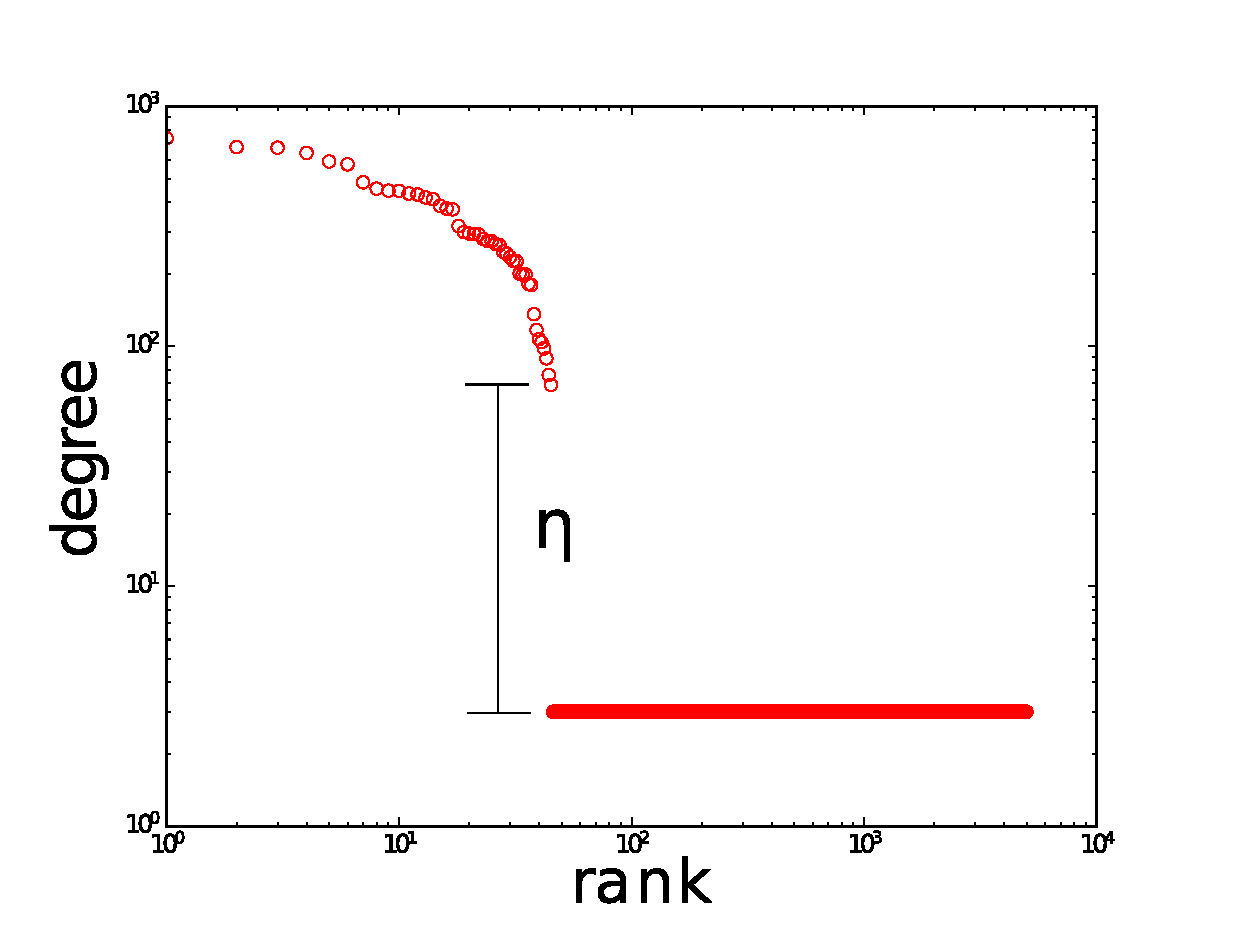
\includegraphics[height=5.5cm]{pygraph/baRank.eps}
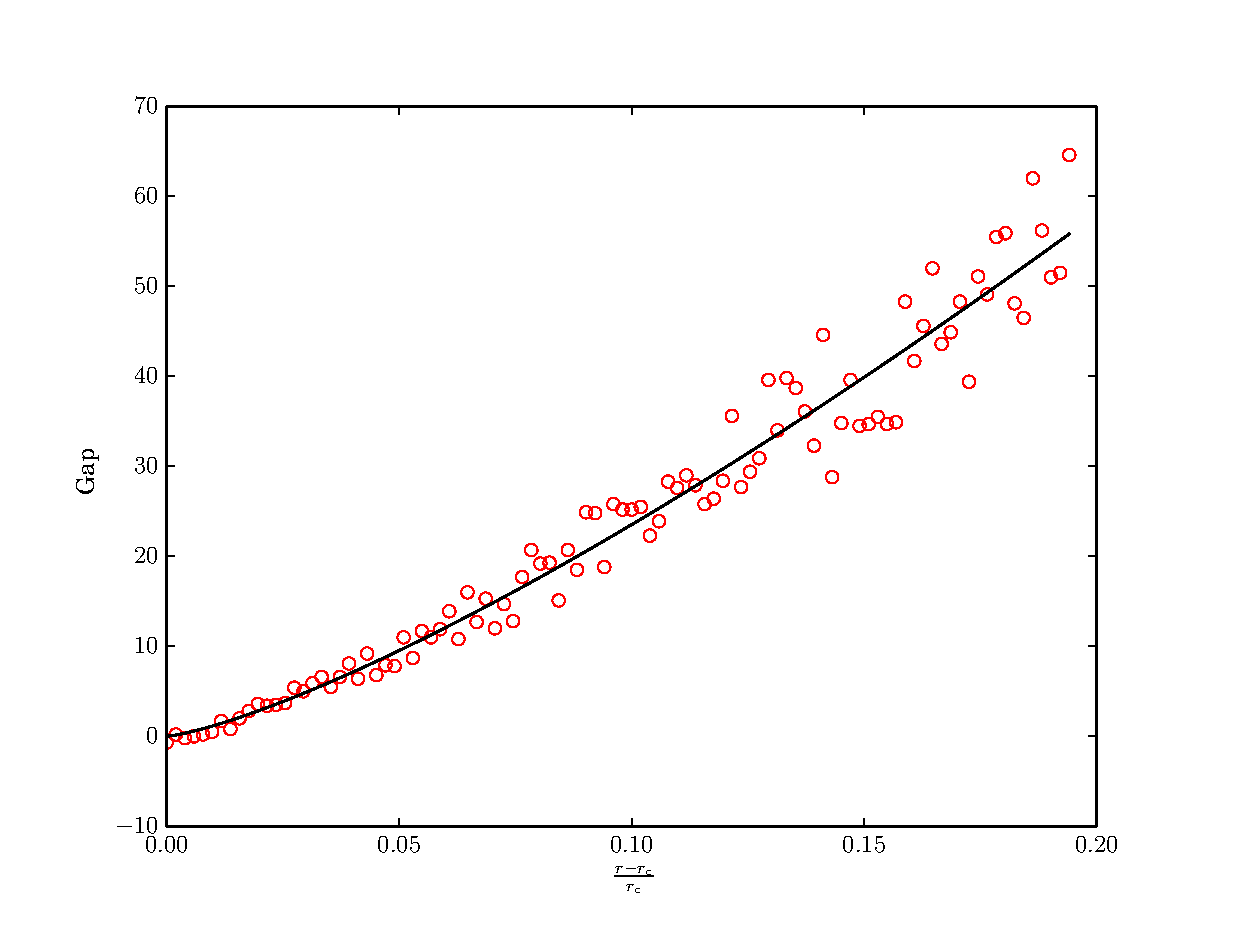
\includegraphics[height=5.5cm]{pygraph/baGap.eps}
\caption{Ранжированое распределение при $r=0.6$. По горизонтальной оси отложено порядковый номер узла, по вертикальной оси отложена степень узла. Изменение величины разрыва}
\end{figure}

Введем новую характеристику сети - величину разрыва $\eta$ рис. \ref{fig:rankDistribution}, расстояние между узлами, ближайшими к разрыву(разница значений степени узла до разрыва и после разрыва). Величина разрыва, указывает по вертикальной оси те значения степеней узлов, которые отсутствуют. 

Как следует из численного моделирования, поведение параметра $\eta$ аналогично поведению параметра порядка в теории фазовых переходов второго рода \cite{Landau}. Как известно, параметр порядка $\eta$, например намагниченность, при приближении температуры к критическому значению $T_c$ уменьшается степенным образом $\eta \sim (r-r_c)^\beta$, где $\beta$ – критический индекс. 
При проведении численного эксперимента были выбраны следующие начальные параметры: количество узлов $N=5000$, начальное количеств узлов $m_0=20$, количество связей у каждого нового узла $m=3$.

На рис. \ref{fig:rankDistribution} показана полученная зависимость $\eta = A \cdot {(r-r_c)}^\beta$, где $\beta \sim 1.3$

\subsection{Коэфициент кластеризации, ассортативность, минимальное среднее расстояние, величина разрыва}
Появление разрыва $\eta$ в распределении степеней узлов $P(k)$ свидетельствует о значительном изменении структуры сети, что не может не сказаться на её характеристиках. Ниже рассмотрено поведение $C$ - коэффициента кластеризации, $A$ - ассортативности и $l$ - минимального среднего расстояния, как функции коэффициента придирчивости $r$, при $r \geq r_c$. Как показал численный эксперимент для сети с $N=5000$ узлов, коэфициент кластеризации $C$, ассортативность $A$, минимальное среднее расстояние $l$ при $r<r_c$ от $r$ не зависит и равна $C_0 \approx 0.01$, $l_0 \approx 3.98$, $A_0 \approx -0.096$, что, как и должно быть, совпадает с расчетами приведенными в \cite{AlBa2,Newman2}. 

При увеличении $r$ от $r_c$ до $r_c + 0.01$ с шагом $0.001$ коэффициент кластеризации увеличивается от $0.04$ до $0.14$, ассортативность уменьшается от $-0.3$ до $-0.6$, среднее минимальное расстояние уменьшается от $3.5$ до $2.9$(согласно рис. \ref{fig:baCharacteristic}). Для нормализации зависимости возьмем отношение параметра к его значению при $r<r_c$, а также приведем зависимости к возрастающим функциям: $A=\frac{A}{A_0}$, $C=\frac{C}{C_0}$, $l=-\frac{l}{l_0}$.

При $r \geq r_c$ такая зависимость появляется, и она оказывается степенной, а именно $C \sim {(r-r_c)}^\alpha$, $A \sim {(r-r_c)}^\gamma$, $l \sim {(r-r_c)}^\sigma$, где $\alpha \approx 0.46155027$, $\gamma \approx 0.26025569$, $\sigma \approx 0.11761072$

\begin{figure}[H]
\label{fig:baCharacteristic}
\centering
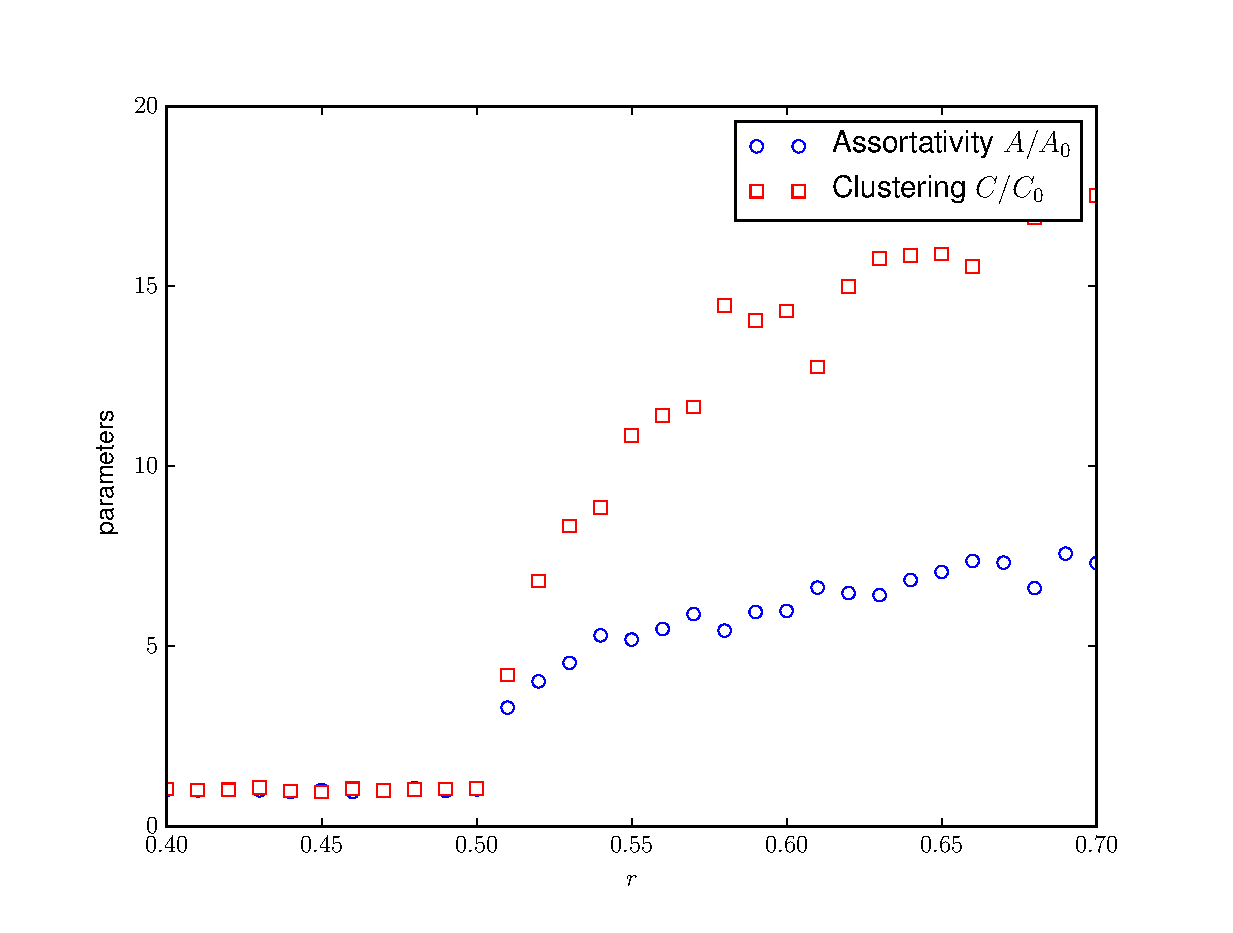
\includegraphics[height=5.5cm]{pygraph/baParams.eps}
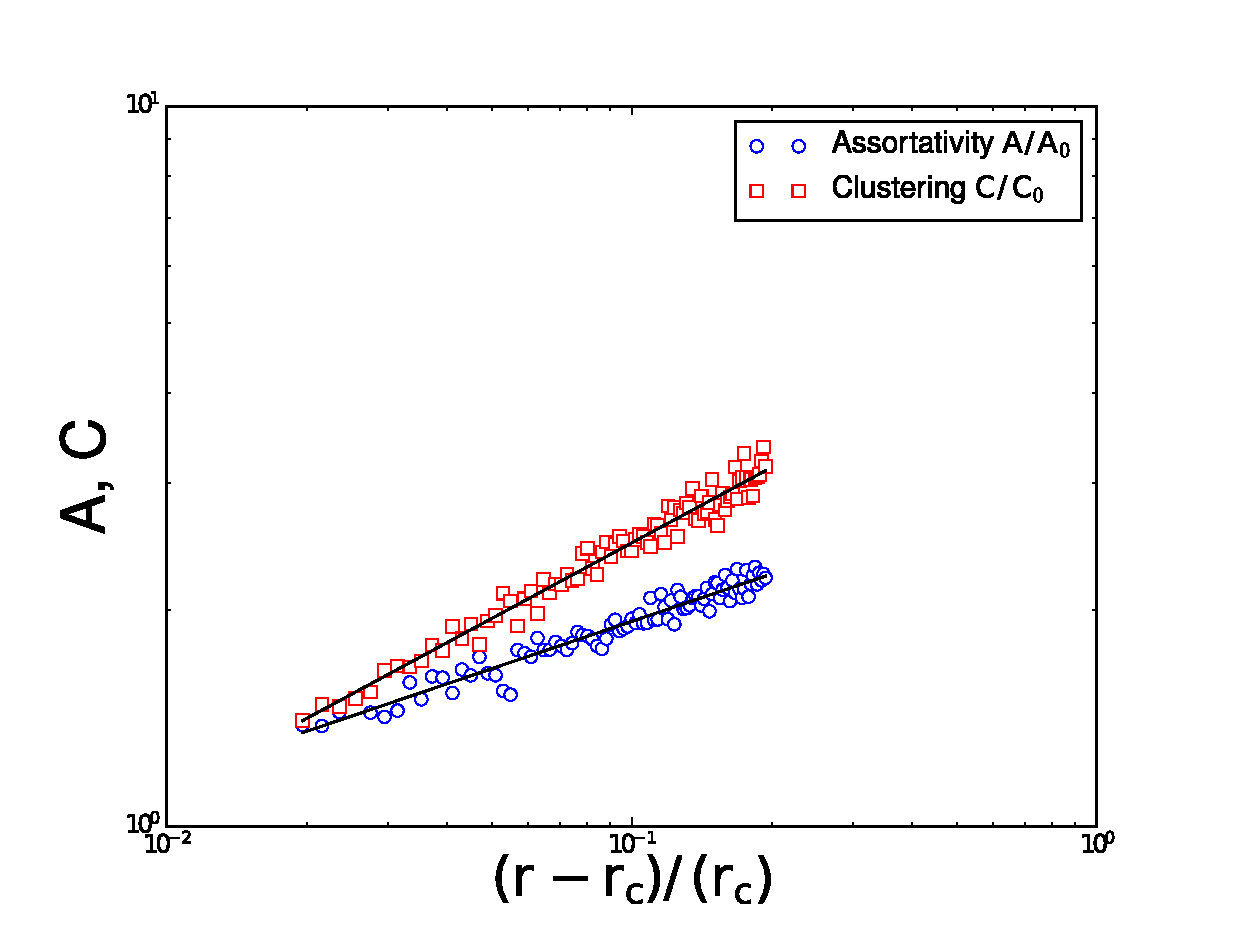
\includegraphics[height=5.5cm]{pygraph/baParamsLog.eps}
\caption{Изменение кластеризации,ассортативности, минимального среднего пути при $r=\lceil 0,51; 0,52 \rceil$ с шагом 0.001}
\end{figure}

% Зависимость этих характеристик $(l,C,A,\eta)$ от $r-r_c$ близка к степенной:

% \begin{equation}
% C \sim 0.28 \cdot (\frac{r-r_c}{r_c})^{0.543} + 0.039
% \end{equation}
% \begin{equation}
% A \sim -0.781 \cdot (\frac{r-r_c}{r_c})^{0.448} - 0.258
% \end{equation}
% \begin{equation}
% l \sim -1.615 \cdot (\frac{r-r_c}{r_c})^{0.516} + 3.551
% \end{equation}
% \begin{equation}
% \eta \sim 472.59 \cdot (\frac{r-r_c}{r_c})^{1.303} + 2.898
% \end{equation}

% Полученные результаты аппроксимируются функцией вида $y \sim ax^b+c$. Фазовий переход описывается функцией вида $y \sim x^b$. Таким образом нашу апроксимирующую функцию можно записать $\frac{y-c}{a} \sim x^b$. Так как нас интересует только поведение функции, можно пренебречь коэффициентом $c$, тоесть сместить наши графики к началу координат. Таким образом можно записать апроксимирующие функции в виде $\frac{1}{a}y \sim x^b$:

% \begin{equation}
% k_1 \cdot C \sim (\frac{r-r_c}{r_c})^{0.543}
% \end{equation}
% \begin{equation}
% k_2 \cdot A \sim (\frac{r-r_c}{r_c})^{0.448}
% \end{equation}
% \begin{equation}
% k_3 \cdot l \sim (\frac{r-r_c}{r_c})^{0.516}
% \end{equation}
% \begin{equation}
% k_4 \cdot \eta \sim (\frac{r-r_c}{r_c})^{1.303}
% \end{equation}

\subsection{Матрица смежности для сети с придирчивостью}
Рассмотрим матрицу смежности $A_{ij}$ для сети с придирчивостью. Для удобства нумерации узлов в матрице смежности будем вести в порядке спадания количества связей. То есть $k_i=\sum\limits_{i}A_{ij}$ не возрастает с увеличением $i$.

\begin{figure}[H]
\label{fig:baRankedMatrix}
\centering
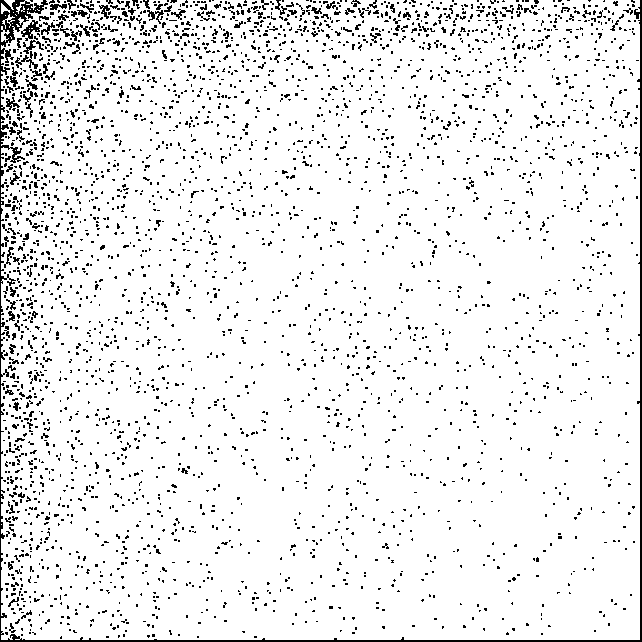
\includegraphics[height=5.5cm]{graphics/bamatrix.png}
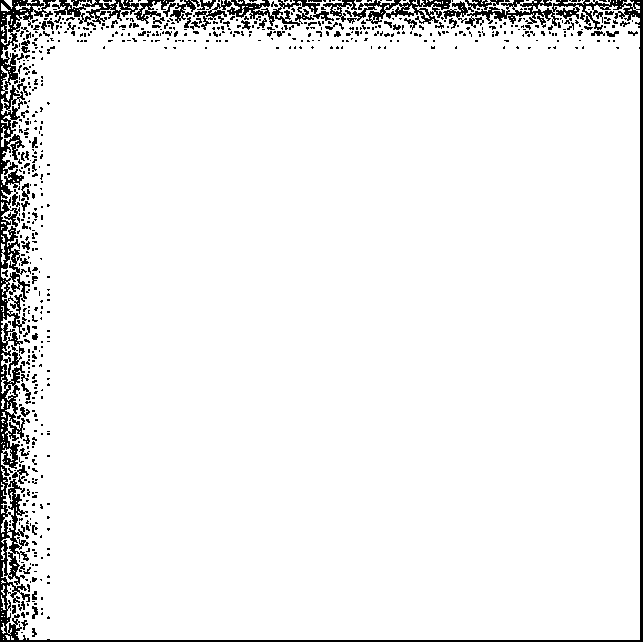
\includegraphics[height=5.5cm]{graphics/bamatrix2.png}
\caption{Матрица смежности при $r=0$ и $r=0.6$}
\end{figure}

Изменение структуры сети при $r \geq r_c$ отражается и на виде матрицы смежности. Для сети с $N=5000$ были построены две матрицы смежности: для $r<r_c$ - рис. \ref{fig:baRankedMatrix} и для $r>r_c$ - рис. \ref{fig:baRankedMatrix}. Для удобвства элементы матрицы смежности $A_{ij}=1$ отображены  в виде черной точки. Обе матрицы были ранжированы, тоесть узлы сети пронумерованы в порядке спадания количества связей $k_i$. Из рис. \ref{fig:baRankedMatrix} можно заметить, что в матрице смежности при $r>r_c$ в правом нижнем углу появляется значительная квадратная область, заполненная 0, тоесть теми парами узлов,которые не связаны друг с другом. Эта область, как показывает исленный эксперимент, прямопропорционально зависит от величины $r$.

Таким образом такие характеристики сети, как коэффициент кластеризации, ассортативность, среднее минимальное расстояние ведут себя аналогично ``параметру порядка'' $\eta$.

\section{Иерархические сети (u,v)-flowers с придирчиостью}
Кроме случайных безмасштабных сетей, построенных по альгоритму Барабши-Альберта(и их обобщений), известен класс простых детерменированных сетей, которые также являются безмасштабными сетями \cite{Rozenfeld2} - Fractal and Transfractal Recursive Scale-Free Networks. В частности это так называемые (u,v)-flowers, рис. \ref{fig:flowerGraph}.

Ниже мы обощим модель Fractal and Transfractal Recursive Scale-Free сетей, введя фактор ``придирчивости'' $r$ и случайность в закон роста сети. Как оказывается в этом случае поведение характеристик сети аналогично фазовому переходу.

\subsection{Алгоритм (u,v)-flowers}
Детерминированные растущие SF-сети, называемые (u,v)-flowers и (u,v)-trees были предложены и исследованы в \cite{Dor1,Rozenfeld1,Rozenfeld2}.

\begin{figure}[H]
\label{fig:flowerGraph}
\centering
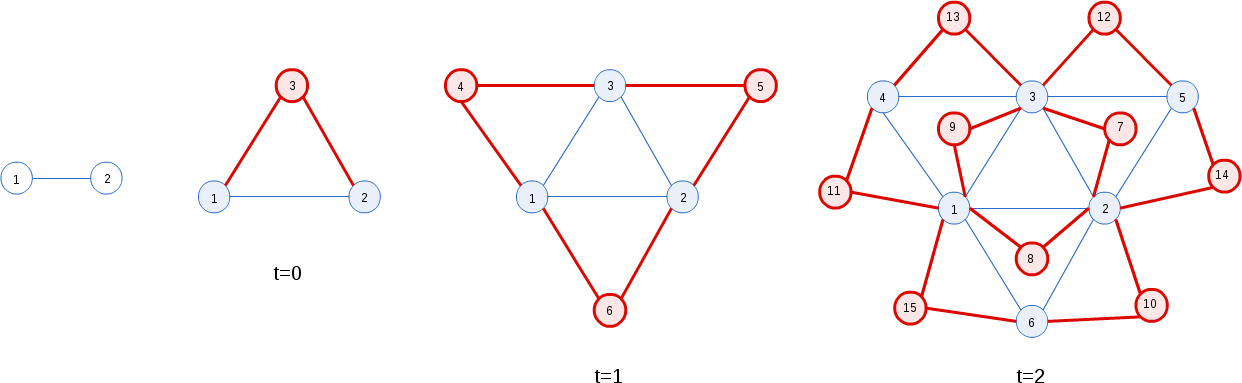
\includegraphics[height=5.5cm]{graphics/hierarhical.png}
\caption{Схема построения (1,2)-flowers на шагах $t=0,1,2$. Утолщенные(красные online) - узлы появивщиеся на данном шаге,не утолщенные (синие online) - узлы, которые появились на предыдущих шагах.}
\end{figure}

Нумерация узлов вообще говоря может быть любой, однако, в рассматриваемом примере можно занумеровать узлы таким образом (рис. \ref{fig:flowerGraph}), что матрица смежности $A_{ij}$ станет наиболее простой. Под простой $A_{ij}$ мы, в данном случае, понимаем такую ее структуру, что наибольшее число наибольших квадратных областей $N \times N$ в нем остаются пустыми.

\begin{figure}[H]
\label{fig:flowerMatrix}
\centering
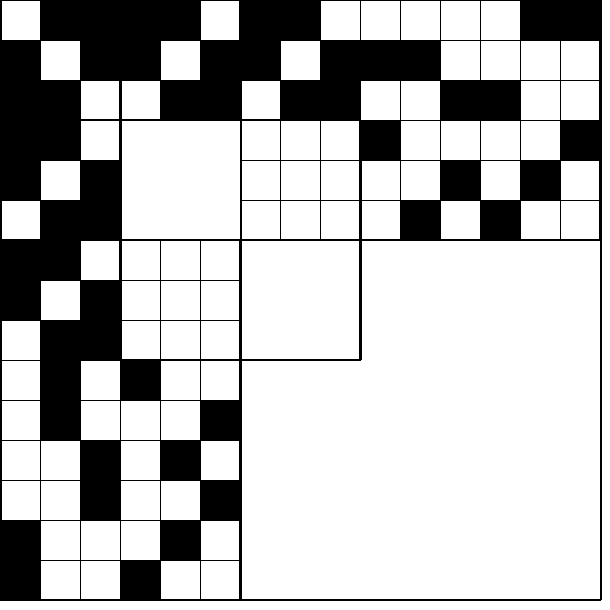
\includegraphics[height=5.5cm]{graphics/first_all.png}
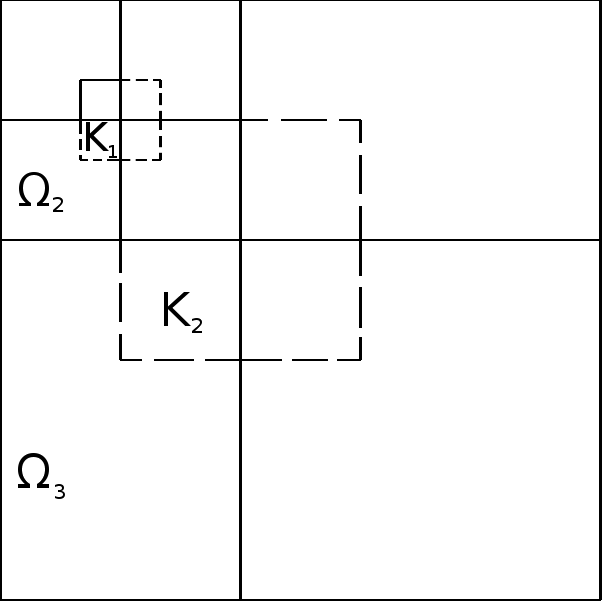
\includegraphics[height=5.5cm]{graphics/second.png}
% 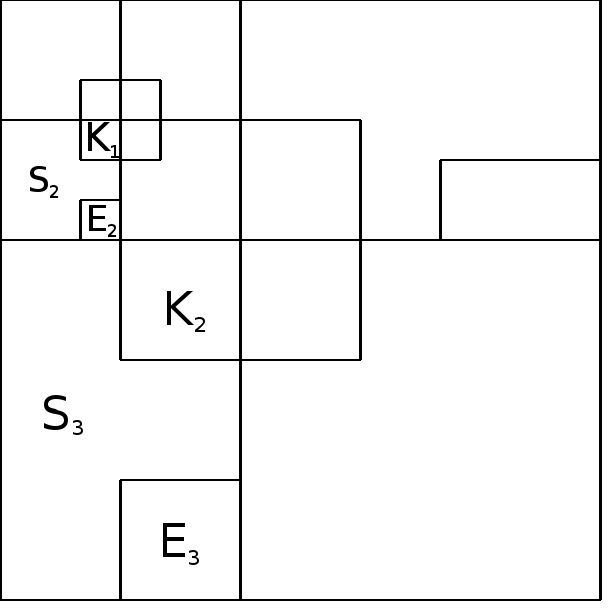
\includegraphics[height=5.5cm]{graphics/third.png}
\caption{Схема матрицы смежости для 3-го шага (1,2)-flower.}
\end{figure}

На рис. \ref{fig:flowerMatrix} - $N \times N$ матрица смежности, где черным обозначены элементы матрицы с $A_{ij}=1$. На первом шаге матрица смежности $\hat{A}$ состоит из $3 \times 3$ элементов(верхний левый угол, шаг $t=0$ на рис. \ref{fig:flowerGraph}). На втором шаге к ней добавляются новые элементы, и матрица состоит из $6 \times 6$ элементов(шаг $t=1$ на рис. \ref{fig:flowerGraph}). На третьем шаге шаге добавляются новые элементы, и матрица состоит из $15 \times 15$ элементов(шаг $t=2$ на рис. \ref{fig:flowerGraph}). Как видно из рис. \ref{fig:flowerMatrix} правый нижний квадрат первого шага свободный от связей и состоит из одного элемента. На втором шаге добавляется правый нижний квадрат, состоящий из $3 \times 3$ элементов, а на третьем из $9 \times 9$ элементов. На рис. \ref{fig:flowerMatrix} белым обозначены места матрицы смежности, где $A_{ij}=0$.

При выбранной нами нумерации появляются дополнительные к построению матрицы смежности в работе \cite{Dor1} области $K_1$, $K_2$, в которых также $A_{i,j}=0$. 

На каждом шаге $t$ имеется $N_t$ узлов и $L_t$ связей \cite{Rozenfeld1}

\begin{equation}
\label{eq:flowerEdgesNodesRecurent}
N_t = (u+v) \cdot N_{t-1}-(u+v), \quad L_t=(u+v)^t
\end{equation}

Т.е. на каждом шаге $t$ появляется $N_t-N_{t-1}$ узлов и $L_t-L_{t-1}$ связей. Например, рис. \ref{fig:flowerGraph}, на шаге $t=1$ появляется 3 узла и 6 связей.

Сделаем замену $(u+v)=w$ и раскроем рекурентные формулы \ref{eq:flowerEdgesNodesRecurent} \cite{Rozenfeld1}:

\begin{equation}
\label{eq:flowerEdgesNodesOpenRecurent}
N_t = \frac{w-2}{w-1} \cdot w^t+\frac{w}{w-1}, \quad L_t=w^t
\end{equation}

На каждом шаге $t$ есть $\Omega_t$ клеток, которые могут быть заполнены – рис. \ref{fig:flowerMatrix}. Их число равно:

\begin{equation}
\label{eq:flowerEmpty}
\begin{split}
\Omega_{t} &=(N_t-N_{t-1}) \cdot N_t-N_{t-2}^2 = \frac{w^3-w^2-1}{w^4}N_t^2 + \frac{w^3-2w^2-2w-2}{w^3}N_t-\frac{2w^2+2w+1}{w^2} = \\
           &= \frac{w^{2t+4}-5w^{2t+3}+8w^{2t+2}-5w^{2t+1}+4w^{2t}+w^{t+5}-3w^{t+4}+4w^{t+2}-w^5}{w^{3} \cdot (w-1)^2}
\end{split}
\end{equation}

Вероятность заполнения ячейки матрицы равна:

\begin{equation}
W_t=\frac{L_t-L_{t-1}}{\Omega_t}=\frac{w^{t+5}-3w^{t+4}+3w^{t+3}-w^{t+2}}{w^{2t+4}-5w^{2t+3}+8w^{2t+2}-5w^{2t+1}+4w^{2t}+w^{t+5}-3w^{t+4}+4w^{t+2}-w^5}
\end{equation}

Так c каждым шагом вероятность падает и матрица смежности становится все более разряженной.
В \cite{Dor1} было показано, что (u,v)-flowers являются безмасштабными сетями. Для изображенного на рис. \ref{fig:flowerGraph} (1,2)-flower распределение узлов по степеням имеет вид $P(k) \sim k^{-(1+\frac{\ln{3}}{\ln{2}})}$. В общем случаи для (u,v)-flowers \cite{Rozenfeld1}

\begin{equation}
P(k) \sim k^{-\alpha}, \quad \alpha = 1+\frac{\ln{(u+v)}}{\ln{2}}
\end{equation}

\subsection{Модификация алгоритма (u,v)-flowers}

Рассмотрим теперь ситуацию, когда при построении (u,v)-flower не все связи реализуются. При чем вероятность нереализованности связи тем больше, чем меньше степени узлов она соединяет.

\begin{figure}[H]
\label{fig:flowerMatrixExceptive}
\centering
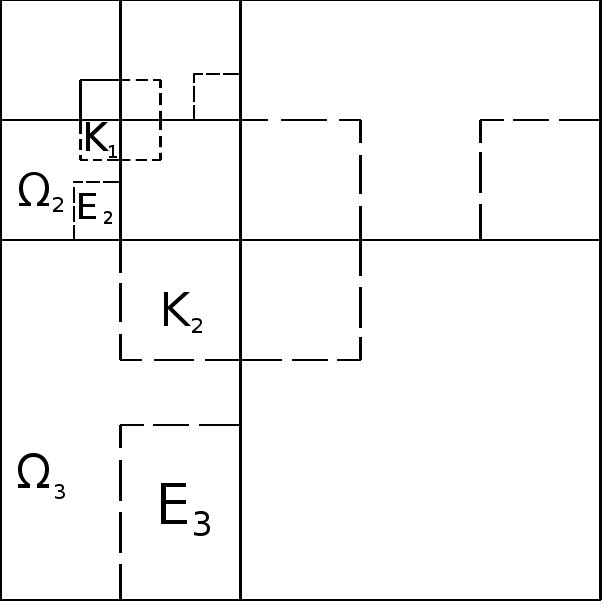
\includegraphics[height=5.5cm]{graphics/third_n.png}
\caption{Схема матрицы смежости для 3-го шага (1,2)-flower.}
\end{figure}

Комрьютерное моделирование проводилось путем заполнения в матрице смежности областей $\Omega_1, \Omega_2...$ с соотетсвующим им количеством связей $L_t$. Таким образом ``придирчивость'' в матрице смежности отображается правыми нижними углами областей $\Omega$. При $r>0$ в правых нижних углах областей $\Omega$ появляются пустые области. В нашем моделировании мы использовали пустые области $E_t$ \ref{fig:flowerMatrix}. Тогда вероятность заполнения ячейки матрицы:

\begin{equation}
W_t=\frac{L_t-L_{t-1}}{\Omega_t-E_t}
\end{equation}

\begin{equation}
E_t= (r \cdot N_{t-1})^2
\end{equation}

\subsection{Функция распределения степеней узлов}

При значение параметра придирчивости $r=0$ предлагаемая модель принимает вид стандартной (u,v)-flowers. Как и в случае с моделью Барабаши-Альберта, в модели (u,v)-flowers присутствует пороговое значения параметра придирчивости $r_c$. При значении параметра придирчивости меньше некоторого порогового $r<r_c$ функция распределения степеней узлов $P(k)$ остается степенной, а сама сеть, тем самым, безмасштабной сетью. При значениях параметра придирчивости больше порогового значения $r \geq r_c$ сеть меняет свою структуру, а именно в сети исчезают узлы со «средним» количеством связей, что мы можем увидеть на рис. \ref{fig:flowerRank}. 

\begin{figure}[H]
\label{fig:flowerRank}
\centering
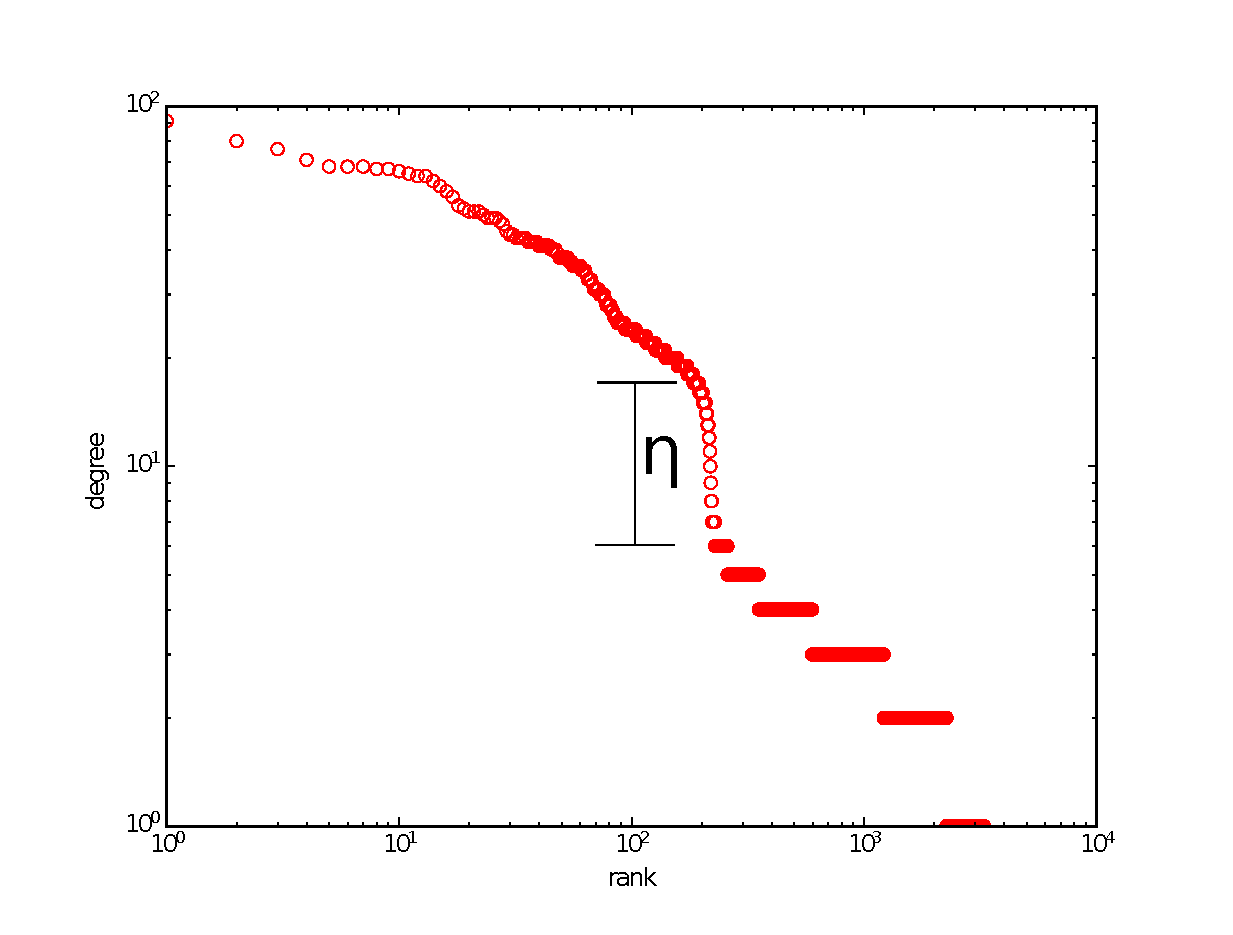
\includegraphics[height=5.5cm]{pygraph/flowerRank.eps}
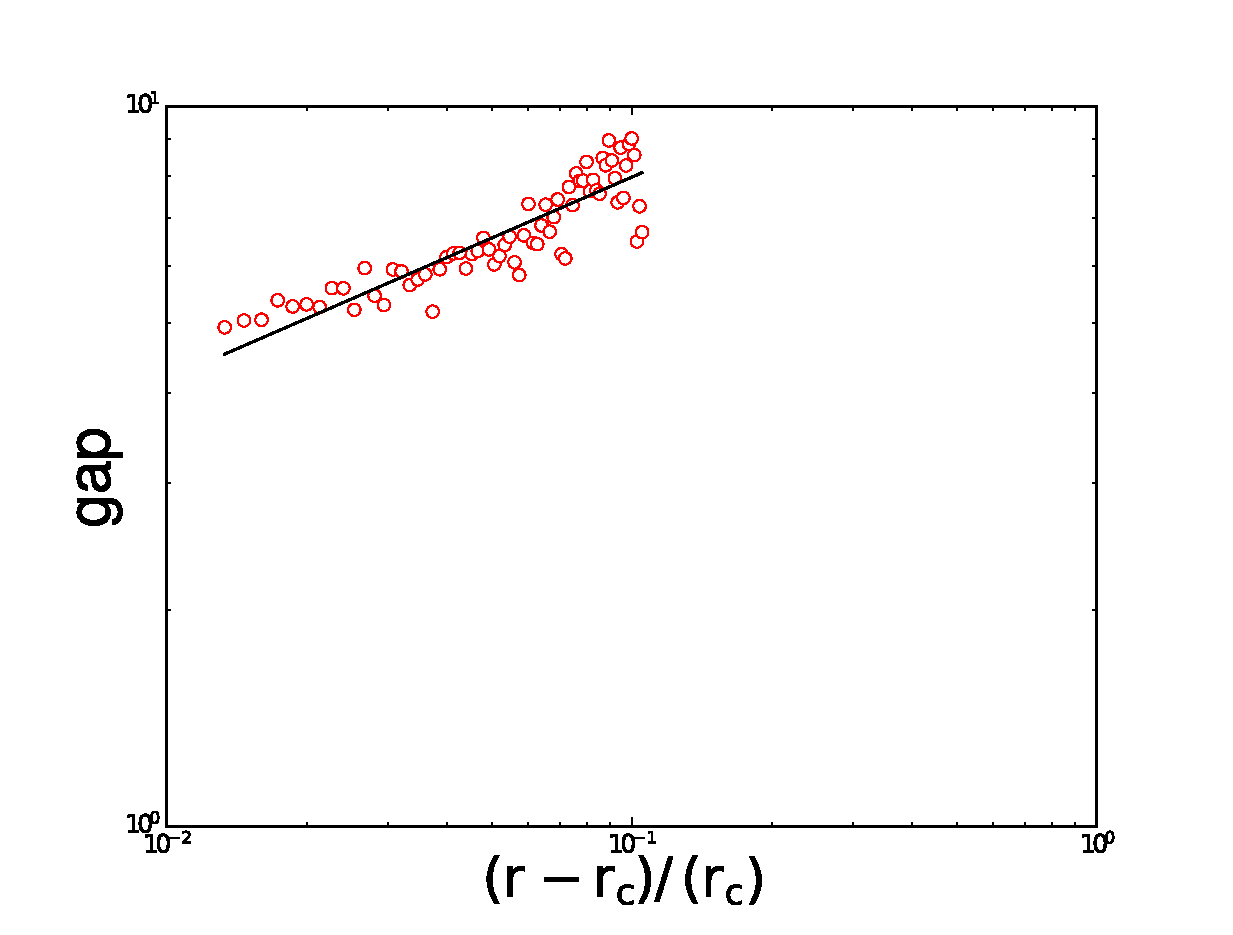
\includegraphics[height=5.5cm]{pygraph/flowerGap.eps}
\caption{Ранжированое распределение узлов}
\end{figure}

Определим пороговое значение параметра придирчивости. Для этого рассчитаем пороговое значение для (u,v)-flowers с 1 по 14 поколение, при этом будем усреднять значения по 10 экспериментам. Как и в модели Барабаши-Альберт с придирчивостью происходит насыщение порогового значения. Для 9 поколения $r_c$ полностью насыщается и мы получаем $r_c=0.91$.

\subsection{Коэфициент кластеризации, ассортативность, минимальное среднее расстояние, величина разрыва}
Появление разрыва $\eta$ в распределении степеней узлов $P(k)$ свидетельствует о значительном изменении структуры сети, что не может не сказаться на её характеристиках. Ниже рассмотрено поведение $C$ - коэффициента кластеризации, $A$ - ассортативности и $l$ - минимального среднего расстояния, как функции коэффициента придирчивости $r$, при $r \geq r_c$, как оказалось при увеличении $r$ от $r_c$ до $r_C + 0.01$ с шагом $0.001$ происходит существенные изменения этих характеристик. Коэффициент кластеризации увеличивается от $0.005$ до $0.007$, ассортативность уменьшается от $-0.18$ до $-0.195$, среднее минимальное расстояние колеблется около значения $1.34$, величина разрыва увеличивается от $4$ до $xxx$(согласно рис. \ref{fig:flowerParam}). 

\begin{figure}[H]
\label{fig:flowerParam}
\centering
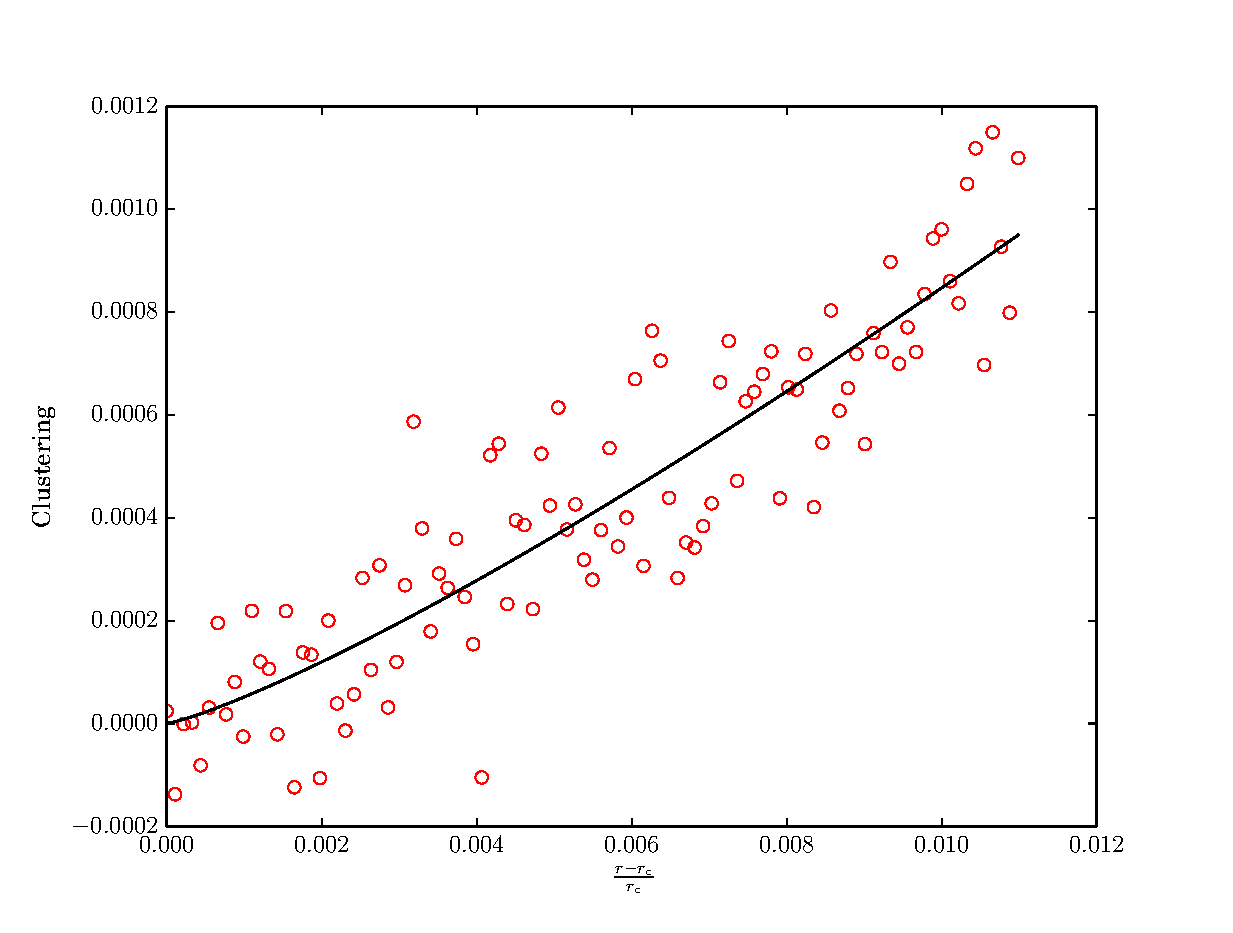
\includegraphics[height=5.5cm]{pygraph/flowerClustering.eps}
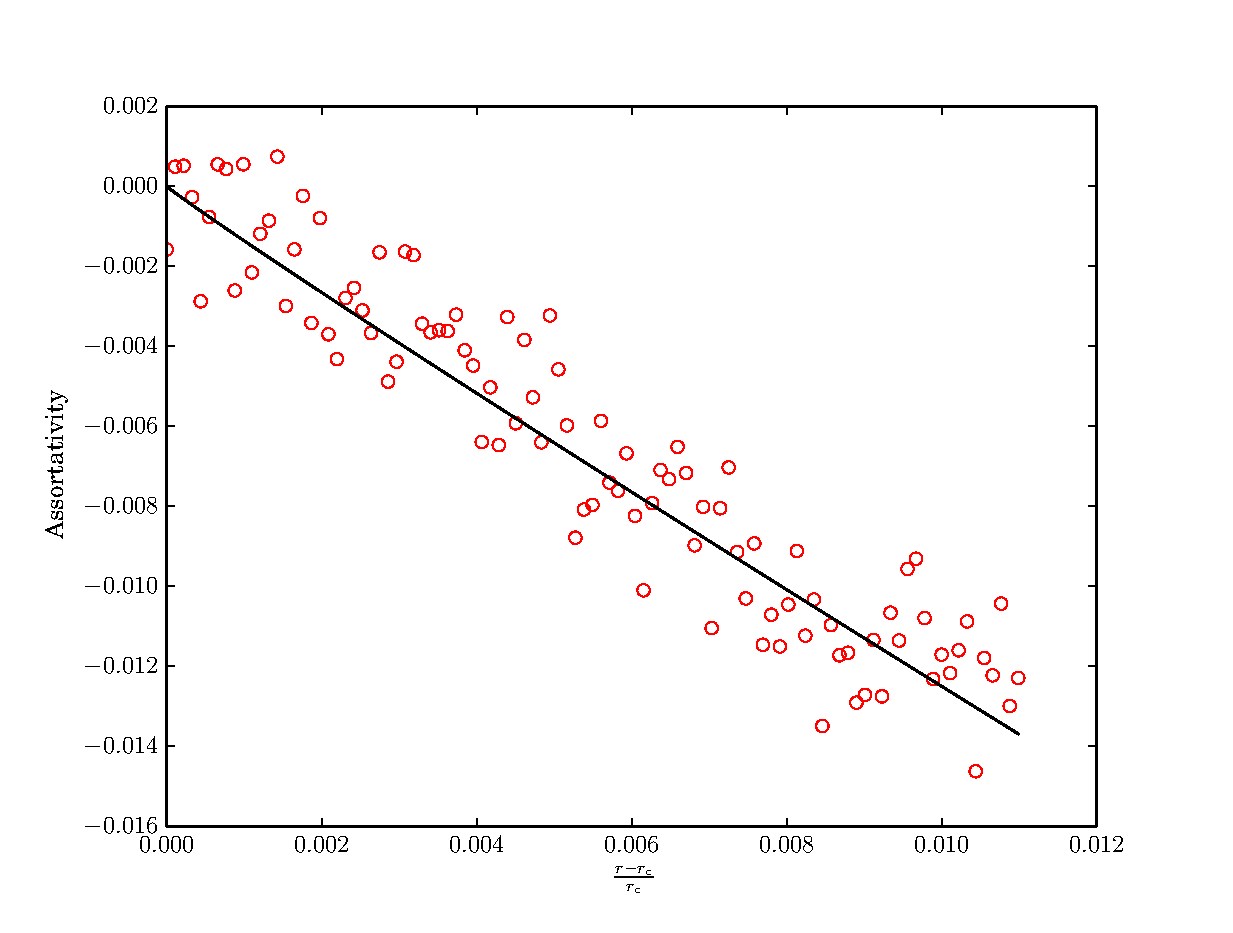
\includegraphics[height=5.5cm]{pygraph/flowerAsort.eps}
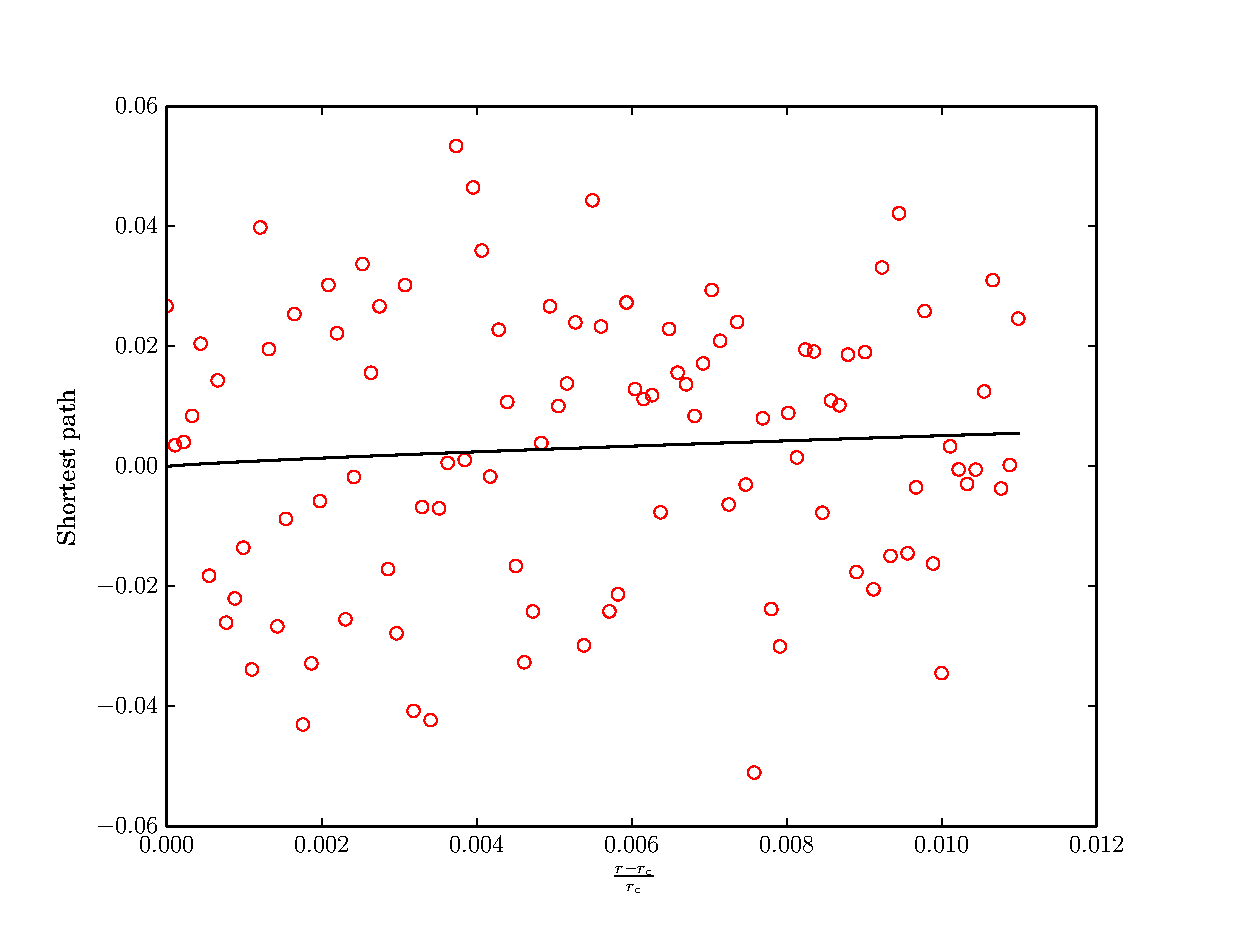
\includegraphics[height=5.5cm]{pygraph/flowerShort.eps}
% 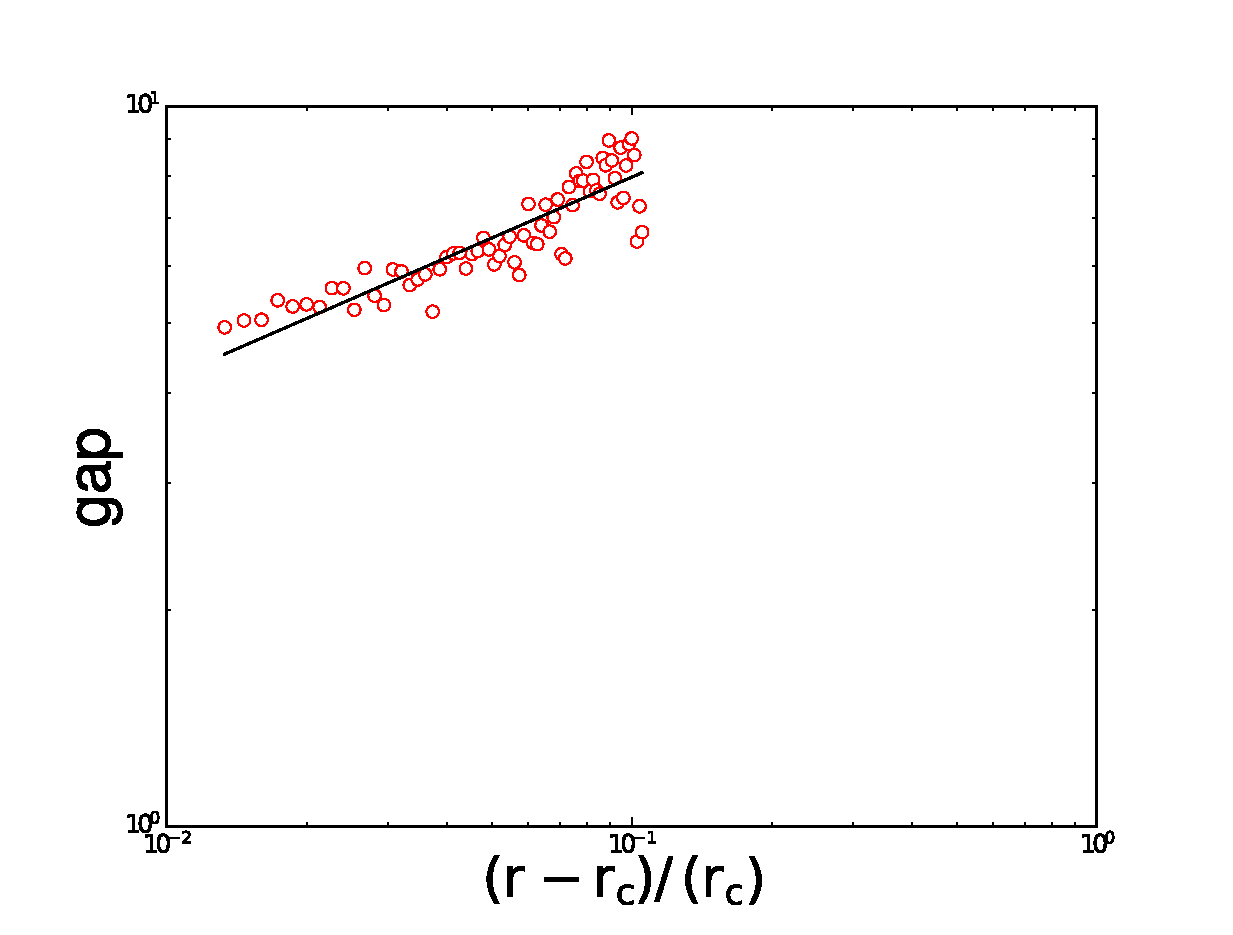
\includegraphics[height=5.5cm]{pygraph/flowerGap.eps}
\caption{Изменение кластеризации,ассортативности, минимального среднего пути при $r=\lceil 0,51; 0,52 \rceil$ с шагом 0.001}
\end{figure}

Зависимость этих характеристик $(C,A,l)$ от $r-r_c$ близка к степенной $C = {r-r_c}^\alpha$, $A = {r-r_c}^\gamma$, $l = {r-r_c}^\sigma$, где $\alpha \sim $, $\gamma \sim $, $\sigma \sim $:


% \begin{equation}
% k_1 \cdot C \sim (\frac{r-r_c}{r_c})^{1.216}
% \end{equation}
% \begin{equation}
% k_2 \cdot A \sim (\frac{r-r_c}{r_c})^{0.963}
% \end{equation}
% \begin{equation}
% k_3 \cdot l \sim (\frac{r-r_c}{r_c})^{0.817}
% \end{equation}
% \begin{equation}
% k_4 \cdot \eta \sim (\frac{r-r_c}{r_c})^{0.256}
% \end{equation}

\section{Заключение}

\section{Литература}

\bibliographystyle{apsrev4-1}
\bibliography{biblio} 

\section*{Пометки}
\begin{enumerate}
\item Битвинес в БА
\item Придирчивостью структурирует сеть( делает из неё иерархическу)
\item Новые графики БА - 5000 узлов, 5 экспериментов, $r=[0.51;0,52]$, шаг 0.001
\item сделать аналогичные расчеты для (2,3)-цветков
\item Объяснить про смещения и т.д. для получения формул.
\item Цветки, нписать про $\eta$
\end{enumerate}

\end{document}

